\graphicspath{{Images/}}

\section{Part 2 - The Effects of Ties}

\textit{Repeated Forward A* needs to break ties to decide which cell to expand next if
several cells have the same smallest f-value. It can either break ties in favor of cells with smaller g-values or in favor of
cells with larger g-values. Implement and compare both versions of Repeated Forward A* with respect to their runtime or,
equivalently, number of expanded cells. Explain your observations in detail, that is, explain what you observed and give a
reason for the observation.}


The source code contains the implementations for both variants of Repeated Forward A*. When the commented section within the main method, responsible for executing both versions across all generated mazes and computing the average time and expanded cells, is uncommented, the ensuing results are as follows.

\begin{figure}[h]
    \centering
    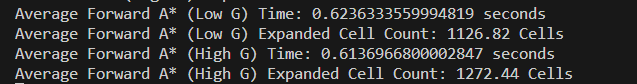
\includegraphics[width=.85\linewidth]{imgs/Results of Both Forward A Methods.png}
    \caption{Comparison of Both Version of Repeated Forward A*}
    \label{fig:my_label}
\end{figure}


Comparing two pathfinder algorithms reveals that the Repeated Forward A* version, which prioritizes higher G-values when breaking ties, demonstrates faster performance. In this context, the G-value (representing the length of the shortest path from the start state to state s as determined by A* search) is a crucial factor. The h-value, or heuristic, remains constant and estimates the distance from state s to the goal state, using Manhattan Distance in this scenario. The f-value, denoted as f(s) := g(s) + h(s), estimates the overall distance from the start state through state s to the goal state.

When faced with multiple cells sharing the smallest f-value, the algorithm has the option to break ties in favor of cells with either smaller or larger g-values. Notably, the version favoring higher G-values proves to be faster. This preference for higher G-values stems from the fact that G-value signifies the length of the shortest path from the start state to state s. Choosing states closer to the start state, rather than the goal state, appears to be advantageous, especially considering that the goal is typically distant from the start state.

The observed outcome, where higher G-values lead to more expanded cells, may be attributed to the algorithm prioritizing exploration of states closer to the start. This approach can be beneficial when the goal is farther away, as it allows the algorithm to efficiently navigate through states that contribute to the initial stages of the path. However, whether favoring higher G-values is preferable depends on the specific characteristics and requirements of the given problem.